% This is file `xampl-thesis.tex',
% generated with the docstrip utility.
%
% The original source files were:
%
% vakthesis.dtx  (with options: `xampl-thesis')
% 
% IMPORTANT NOTICE:
% 
% For the copyright see the source file.
% 
% Any modified versions of this file must be renamed
% with new filenames distinct from xampl-thesis.tex.
% 
% For distribution of the original source see the terms
% for copying and modification in the file vakthesis.dtx.
% 
% This generated file may be distributed as long as the
% original source files, as listed above, are part of the
% same distribution. (The sources need not necessarily be
% in the same archive or directory.)
% Існують кілька опцій, які необхідно вказувати як факультативний
% аргумент команди \documentclass. Наприклад, для докторської
% дисертації необхідно написати
% \documentclass[d]{vakthesis}

% Налагодження кодування шрифта, кодування вхідного файла
% та вибір необхідних мов
\documentclass[14pt]{vakthesis}
\usepackage{extsizes}
\usepackage{cmap} % для кодировки шрифтов в pdf
\usepackage[T1,T2A]{fontenc}
\usepackage[utf8]{inputenc}
% \usepackage{luaotfload}
%\usepackage[EU2]{fontenc}
%\usepackage{lmodern}

\usepackage[english,ukrainian,russian]{babel}

%usepackage{libertine}
% \usepackage[letterspace=-36]{microtype}

% Підключення необхідних пакетів. Наприклад,
% Пакети AMS для підтримки математики, теорем, спеціальних шрифтів

\usepackage{packages}
\allowdisplaybreaks


% Налагодження параметрів сторінки (зокрема берегів).
% Наприклад, за допомогою пакета geometry
\usepackage{geometry}
\geometry{hmargin={30mm,15mm},lines=29,vcentering}

% Якщо потрібно працювати лише з деякими розділами
%\includeonly{xampl-ch1,xampl-bib}

% Інформація про використані пакети тощо.
% Може знадобитися для відлагодження класу документа
%\listfiles
\makeatletter
\let\@Asbuk\@Alph
\let\@asbuk\@alph
\makeatother


% Титульна сторінка
\makeatletter
\def\onesupervisorname{Науковий\
    керівник}%
  \def\manysupervisorsname{Наукові\
    керівники}
\makeatother 

%\makeatletter
%\def\@maketitle{%
%  {\scshape
%   \@ifundefined{@institution@office}{\relax}{\@institution@office\par}
%   \@institution\par}
%  \vspace{\stretch{3}}%
%  {\raggedleft \@ifundefined{@secret}{}{\@secret\hfill}%
%     На правах\
%     рукопису \par}%
%  \vspace{\stretch{2}}%
%  {\bfseries\expandafter\emphsurname\@author \par}%
%  \vspace{\stretch{2}}%
%  {\raggedleft \CYRU\CYRD\CYRK\ \@udc \par}%
%  \vspace{\stretch{1}}%
%  {\large\bfseries\scshape \@title \par}%
%  \vspace{\stretch{2}}%
%  \@specialitycode\ --- \@specialityname\par
%  \vspace{\stretch{2}}%
%  Дисертація\
%    на\ здобуття\
%    вченої\
%    ступені\linebreak[1]%
%    \degreename\cyra\
%    \@science\par%?\linebreak[1]%
%  \vspace{\stretch{2}}%
%  {\raggedleft
%   \let\\\@format@person
%   \ifx\@supervisors\@empty
%     \hbox{}\hbox{}\hbox{}
%   \else
%     \@supervisors@caption\@supervisors\relax
%   \fi
%   \par}%
%  \vspace{\stretch{3}}%
%  \@town\ --- \@year}
%\def\@supervisors@caption{%
%  \ifnum\value{@supervisors@count}>1
%    \manysupervisorsname:%
%  \else
%    \onesupervisorname
%  \fi}
%\def\@format@person#1#2{\linebreak[4]%
%  \textbf{#1}, \linebreak[1]\@@format@person#2,,\@nil
%  \futurelet\next\@delimit@person}
%\def\@@format@person#1,#2,#3\@nil{#1%
%  \if\relax#2\relax\else, \linebreak[0]#2\fi}
%\def\@delimit@person{\ifx\relax\next\else,\fi}
%\def\emphsurname#1 #2{\textsc{#1} #2}
%\makeatother 

% Локальні означення
%\hyphenpenalty=10000

% NAMES
%% Переопределение именований %%%
\renewcommand{\abstractname}{Анотація}
% \renewcommand{\alsoname}{см. также}
\renewcommand{\appendixname}{Додаток}
\renewcommand{\bibname}{СПИСОК ВИКОРИСТАНИХ ИСТОЧНИКОВ}
% \renewcommand{\ccname}{исх.}
%\renewcommand{\chaptername}{Раздел}
\renewcommand{\chaptername}{РАЗДЕЛ}
\renewcommand{\contentsname}{СОДЕРЖАНИЕ}
% \renewcommand{\enclname}{вкл.}
\renewcommand{\figurename}{Рис.}
% \renewcommand{\headtoname}{вх.}
\renewcommand{\indexname}{Предметный указатель}
\renewcommand{\listfigurename}{Список рисунков}
\renewcommand{\listtablename}{Список таблиц}
%\renewcommand{\pagename}{Стр.}
\renewcommand{\partname}{Часть}
%\renewcommand{\refname}{СПИСОК ИСПОЛЬЗОВАННЫХ ИСТОЧНИКОВ}
% \renewcommand{\seename}{див.}
\renewcommand{\tablename}{Табл.}
% \renewcommand{\proofname}{Доказательство}
% \renewcommand{\algorithmcfname}{Алгоритм}% Update algorithm name
%
%% Настройка разделителей в содержании
%\renewcommand{\cftpartleader}{\cftdotfill{\cftdotsep}} % for parts
%\renewcommand{\cftchapleader}{~~\cftdotfill{\cftdotsep}} % for chapters
%\renewcommand{\cftsecleader}{\cftdotfill{\cftdotsep}} % for sections, if you really want! (It is default in report and book class (So you may not need it).


% COMMANDS
%
\newcommand{\bs}[1]{\ensuremath{\boldsymbol{#1}}}
\newcommand{\len}[1]{|#1|}
\newcommand{\pto}{\dashrightarrow}
\newcommand{\diver}{\!\uparrow}
\newcommand{\conver}{\!\downarrow}
\newcommand{\conveq}{\mathrel{\downarrow\!=}}
\newcommand{\var}[1]{\mbox{\texttt{#1}}}
%
\newcommand{\down}{\conver}
\newcommand{\downeq}{\conveq}
\newcommand{\pmaps}{\pto}
\newcommand{\conv}{\conver}


%=======================================
%

% Environments
% \theoremstyle{plain}
\newtheorem{problem}{Задача}[chapter]
\newtheorem{example}{Пример}[chapter]
\newtheorem{proposition}{Предложение}[chapter]
\newtheorem{corollary}{Следствие}[chapter]
\newtheorem{lemma}{Лемма}[chapter]
\newtheorem{theorem}{Теорема}[chapter]

% \theoremstyle{definition}
\newtheorem{definition}{Визначення}[chapter]

% \theoremstyle{remark}
\newtheorem{remark}{Замечание}[chapter]
%================================================
% 
 

\begin{document}


% \setdefaultleftmargin{0pt}{}{}{}{}{}

% Назва дисертації
\title{Математичні імітаційні моделі для забезпечення узгодженості для розподілених сховищ даних}
% Прізвище, ім'я, по батькові здобувача
\author{Жолткевич Галина Григоріївна}
% Прізвище, ім'я, по батькові наукового керівника/консультанта
\supervisor{Рукас Кирило Маркович}
% Науковий ступінь, вчене звання наукового керівника/консультанта
           {доктор технічних наук, доцент}
% Спеціальність
%\speciality{01.05.02}
% Варіант із вказуванням факультативних аргументів
\speciality[Математичне моделювання та обчислювальні методи]{01.05.02}[технічних наук]
% Індекс за УДК
\udc{004.042/519.713.2}
% Установа, де виконана робота, і місто
\institution{Міністерство освіти і науки України \linebreak Харківський національний університет імені~В.Н.~Каразіна}{Харків}
% Рік, коли написана дисертація
\date{2019}

% Тут буде титульна сторінка
\maketitle

% Зміст
\tableofcontents

\chapter*{Вступ}

\paragraph{\bfseries Актуальність теми.}

В наше сьогодення інноваційні технології з'являються дуже швидко, а існуючі розвиваються з неймовірною швидкістю. Гіперлуп, багаточисленні дослідження космосу, наукові роботи в інших галузях, таких, 
як медицина, зелені мережі, а також, більш побутові, але все ще такі потрібні технології, такі, як 
комунікації, транспорт, розумні будинки... Не можна нехтувати тим фактом, що всі ці системи потребують
більшої гнучкості, швидкості, надійності та засобів для зберігання інформації також надійно та швидко і доступно, а інколи навіть доступність має бути майже у будь-якій точці земної кулі.
Тому одним з найважливіших компонентів для багатьох таких систем є швидке і надійне розподілене сховище.
В 21 столітті термін "розподілене сховище" становиться вже звичним. Деякі сховища збільшують кількість вузлів, деякі - ні. Причиною цьому є те, що багато з таких систем потребують сильної узгодженості даних. Але якщо збільшувати кількість вузлів для сховища, консистентність падає дуже швидко. А для деяких систем це важлива частина для їх стабільної роботи.

Бо є дуже відома CAP-теорема, яка стверджує, що неможливо одночасно задовільнити всі три 
характеристики для сховища, узгодженість (consistency), доступність (availability), 
стійкість до розділення (partition tolerance).

Ми не збираємося оскаржувати цю теорему, але робимо спробу обійти цю проблему. Механізм для цього і буде темою для цієї роботи.

\paragraph{\bfseries Взаємозв'язок роботи з науковими програмами, планами, темами.}
Диссертаційна робота виконана згідно з планом \linebreak
наково-дослідницьких работ Харківського Національного Університету ім.В.Н.Каразіна в рамках теми "Математичне и комп'ютерне моделювання процесів в розподілених базах даних" 
(номер государственной регистрации 0112U002098).


\paragraph{\bfseries Мета і завдання дослідження.}
Метою роботи являється побудува імітаційних та математичних моделей для механізму
підтримки сильної узгодженості у розподілених сховищах даних, проведення експериментів, оцінювання складності імітаційних моделей, побудува метрик, за якими можна дослідити складність даних моделей, а також розробка
обчислювальних методів для сформованого механізму. Це дозволить оцінити, наскільки можна розширити будь-яку розподілену систему і сформує методи для коректної роботи за такими умовами.

Для досягнення цієї мети у роботі розв'язані наступні задачі:
\begin{enumerate}[widest=9999,itemindent=*,leftmargin=0pt]
\item дослідження властивостей розподілених систем, зокрема, розподілених сховищ
\item дослідження критеріїв розподілених баз даних: узгодженості, доступності, стійкості
\item аналіз типів узгодженості
\item аналіз алгоритмів розповсюдження реплік
\item побудова математичної моделі для розподіленого сховщиа даних
\item доказ гіпотези про швидкість розповсюдження реплік
\item модель балансування узгоджених реплік
 
(пояснити які задачі були виконані шоб привести до актуальності задачі в цілому)

\end{enumerate}

\chapter{Теоретичні основи розподілених баз даних та цілісності даних}

Наскільки нам відомо, відповідно до CAP-теореми можна задовільнити тільки будь-які дві з трьох характеристик
для розподіленого сховища данихю
В цьому розділі розглядається можливість досягнути компромісу та забезпечити консистентні відповіді 
від бази даних, не втрачая доступності і стійкості для будь-якого сховища даних.
У цій частині ми пояснюємо гіпотезу, а далі проводимо дослідження, наскільки вдастся досягнути узгодженості завдяки
представлением маніпуляціям.

То ж давайте підійдемо ближче до суті.

Нехай у нас є розподілене сховище даних, що має N вузлів. Зараз ми не враховуємо функцію кожного вузла (мастер чи слейв) і 
вважаємо що кожний вузол приймає запити на читання і запис. Дозвольте нам сконцентруватися на механізмі обробки запитів.

Наша гіпотеза полягає в тому, що у сховищі даних узгодженість після запита на запис досягне достатнього значення с такою швидкістю, що сховище не встигне втратити доступності даних, і є можливість одночасно підтримувати узгодженість, коли відповіді на запити будуть балансувати тільки між вузлами, узгодженими між собою у даний момент часу, з достатньою швидкістю, у відповідь на запит конкретного юніта даних.
Мета цієї роботи полягає у оцінюванні значення узгодженості і доступності даних як результат роботи такого механізму, та алгоритму реалізації.

У цій частині, для того, щоб оцінити ефективність такого алгоритму, значення узгодженості і доступності, розглянемо ближче концепт цього рішення.
\section{Розподілені бази даних та їх типи узгодженості}

Розподілена база даних (або розподілене сховище даних) — це сукупність логічно взаємопов'язаних баз даних, розподілених у комп'ютерній мережі. Логічний зв'язок баз даних в розподіленій базі даних забезпечує система управління розподіленою базою даних, яка дозволяє управляти розподіленою базою даних таким чином, щоб створювати у користувачів ілюзію цілісної бази даних. 


Для будь-якої розподіленої бази даних існують такі властивості, встановлених К.Дейтом (див. \cite{bib:database_principles} :
\begin{itemize}
 \item Локальна автономія. Вона означає, що управління даними в кожному вузлі виконується локально і незалежно від інших вузлів системи
 \item Незалежність вузлів. Вважається, що в ідеальній системі всі вузли рівноправні і незалежні, а бази даних є рівноправними постачальниками інформації в загальний інформаційний простір.
 - Прозорість розміщення даних. Користувач не мусить знати де розміщені дані. Під час роботи створюється враження, що дані знаходяться саме на його комп’ютері.
 - Прозора фрагментація. Ця властивість трактується, як можливість створення фізично розподілених даних, які логічно утворюють єдине ціле. Допускається горизонтальна та вертикальна фрагментація.
 - Прозорість тиражування. Забезпечує тиражування (перенос змін) об’єктів первинної бази даних в усі вузли її розміщення внутрішньосистемними засобами.
 - Обробка розподілених запитів. Означає виконання операцій, сформованих, в рамках звичайного запиту на мові SQL.
 - Обробка розподілених транзакцій. Забезпечує виконання операцій з одночасним забезпеченням цілісності і узгодженості даних, шляхом використання двофазового протоколу фіксації транзакцій.
 - Незалежність від обладнання. Для оснащення вузла можуть використовуватися комп’ютери різних марок і виробників.
 - Незалежність від операційних систем. Передбачає допустимість взаємодії різноманітних операційних систем у різних вузлах розміщення розподіленої бази даних.
 - Прозорість мережі. Забезпечує будь-які протоколи в локальній обчислювальній мережі, яка обслуговує розподілену базу даних.
 - Незалежність від типу баз даних. Допускає співіснування різних систем керування базами даних.
 - Неперервність операцій. Дані доступні завжди, а операції над ними проводяться неперервно.

\end{itemize} 
http://citforum.ru/database/kbd96/45.shtml
Також для розподіленої бази даних існують три найважливіші парадигми, за допомогою яких підтримується ефективна робота для користувача:
\begin{itemize}
\item[Цілісність] Це складна проблема в розподіленій системі даних. Її рішення - синхронна і узгоджена зміна даних у кількох локальних базах даних, які скаладають розподілене сховище, і воно досягається застосуванням протокола фіксації транзакцій. Але це може застосовуватися у випадку, якщо база даних однородна. Якщо розподілена БД неоднородна, для цього використовують механізми розподілених транзакцій. Проте, це можливо при підтримці ХА-інтерфейсу учасниками обробки розподіленої транзакції, які функціонують на вузлах системи,   Это, однако, возможно, если участники обработки распределенной транзакции - СУБД, функционирующие на узлах системы. ХА-інтерфейс визначений в специфікації DTP консорціума X/Open. Нині XA-інтерфейс підтримується CA-OpenIngres, Informix, Microsoft SQL Server, Oracle, Sybase.
Якщо в розподіленому сховищі передбачено тиражування даних, це одразу пред'являє жорсткі  вимоги до підтримки цілісності на вузлах, куди направляються потоки тиражованих даних. То ж конфлікти щодо змін, які необхідно відслідковувати, неминучі. 
\item[Узгодженість] Як і у всіх інших розподілених систем, одним з основних компонентів цілісності даних (цілісності системи) є узгодженість - гарантія того, що усі вузли бачать однакові дані на будь-який момент часу.
Підтримка узгодженості в базах даних є ключовою при стабільній роботі розподіленого сховища даних. 
За узгодженістю слідують доступність даних (в будь-який момент кліент може отримати дані зі сховища або відповідь про те, що їх нема, за розумний обсяг часу) і стійкість до розділення системи (не зважаючи на розділення на ізольовані секції або втрати зв'язку з частиною вузлів, система не втрачає стабільність і здатність коректно відповідати на запити).

\end{itemize}

{\bfseries{red} Реплікація з книжки Таненбаума}
Є відома теорема CAP, яка наголошує, що з трьох властивостей (узгодженість (consistency), доступність (availability), стійкість до розділення (partition tolerance)) неможливо забезпечити більше двох в одній і тий самій конфігурації системи: наприклад, якщо забезпечити узгодженість, втратиться одна з двох інших властивостей. 

Крім того, в цій роботі важливо зазначити, що розділяють наступні моделі узгодженості:

\begin{itemize}
\item Сувора узгодженість (несуперечливість) (Strong Consistency) - на будь-який запит на читання елемента даних $x$ сховище дає значення, які відповідає наойновішої версії. Це найжорсткіша, але модель несуперечливості для підтримки абсолютної узгодженості, і її забезпечення до втрачання вкличини доступності для даної конфігурації сховища даних.

\item Послідовна несуперечливість (sequential consistency) - результат будь-якої дії такий же, якщо б операції читання та запису всіх процесів у сховище даних виконувались би в деякому послідовному порядку і притому операції кожного окремого процесу виконувались би у порядку, визначеного його програмою. Тобто будь-яке правильне чередування операцій читання и запису є допустимим , але всі процеси бачать одне и те ж чередування операцій.

\item Причинна несуперечливість (causal consistency) - операції на запис, які потенціально зв'язані причинно-наслідковим зв'язком, повинні  обслуговуватися всіма процесами в одному і тому ж порядку, а паралельні записи можуть параллельно обслуговуватися на разних вузлах в різному порядку.

\item Несуперечливість FIFO. Операції запису, які здійснюються поодиноким процесом, розглядаються іншими процесами в тому порядку, в якому вони здійснюються, але операції запису з різних процесів, можуть спостерігатися різними процесами у різному порядку.

\item Потенціальна несуперечливість - при відсутності змін всі репліки поступово стають несуперечливими. Такі моделі використовуються, коли клієнт запрошує завжди одну й ту ж репліку та записи в таке сховище виконуються нечасто.


\end{itemize}

Забезпечення суворої узгодженості - занадто дорога модель для будь-якої розподіленої бази даних, хоча деякі бази це забезпечують, для яких застосування такої моделі - сувора технічна вимога, що випливає з бізнес-логіки продукту, де така база використовується.
Але такі конфігурації розподілених БД втрачають значення іншої характеристики - доступності даних, бо для великих БД потрібно багато часу, щоб досягнути суворої несуперечливості і клієнт змушений чекати, щоб мати гарантію на отримання несуперечливих актуальних даних.

Ми намагаємося знайти компроміс, щоб максимально близько реалізувати таку модель без втрачання доступності і стійкості до розділення розподіленої бази (див. модель реалізації  у наступних частинах).

\section{Використання різних моделей несуперечливості у реалізаціях розподілених баз даних}
\section{Балансування навантаження}

Балансувальник навантаження - це метод, який дозволяє розподіляти задачі між мережевими пристроями з метою оптимізації використання ресурсів, збереження часу відопвіді на запити, горизонтального масштабування кластеру та забезпечення відмовостійкості розподіленої системи. Прикладами пристроїв, до яких може бути застосований цей метод, є серверні кластери, проксі-сервери, межмережеві екрани, комутатори, сервери інспектування вмісту, сервери DNS, мережеві адаптери. Балансувальник запиту може бути застосований у різних цілях, також деякі реалізації балансування - проекти з відкритими джерелами, які дозволяють дописати необхідний функціонал для перенаправлення запитів за необхідним алгоритмом, допрацювати існуючі алгоритми та інше (HAProxy, Nginx, Seesaw, Zevent, Neutrino, Traefik, тощо https://geekflare.com/open-source-load-balancer/).
\begin{figure}
\centering
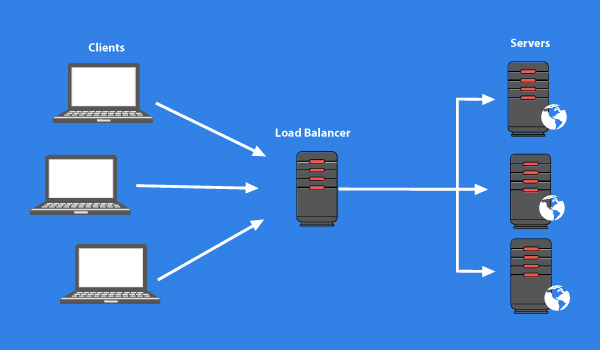
\includegraphics[width=\linewidth]{images/load-balancing-general.jpg}
     \caption{Загальна архітектура балансування навантаження.}
     \label{fig:lb_general}
\end{figure}

Малюнок \ref{fig:lb_general} демонструє загальний механізм роботи  балансувальника навантаження: запит приходить спочатку на проміжний вузел (або кластер) і далі  перенаправляється на один з вузлів в системі, який спроможний відповісти на запит клієнта. Періодично балансувальник робе так званий "healthcheck", щоб вчасно мати знання про те, які вузли зможуть відповісти на запит.
Балансування може здійснятися за різними додатковими характеристиками: запит відправиться на найбільш незайнятий вузел, на вузел, який за показниками процесора на даний момент часу має не завантажений процесор, тощо. 

Алгоритми балансування навантаження загалом можна класифікувати наступним чином (Малюнок \ref{fig:lb_classification}):

\begin{figure}
\centering
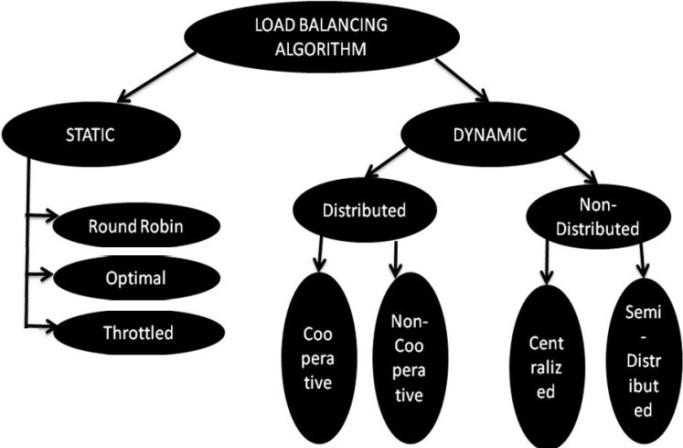
\includegraphics[width=\linewidth]{images/Classification-of-load-balancing-algorithms-in-cloud.png}
     \caption{Класифікація алгоритмів балансування навантаження.}
     \label{fig:lb_classification}
\end{figure}

Ці алгоритми спершу розділяють на статичні і динамічні:

\begin{enumerate}
\item Статичне балансування. В цьому підході балансування навантаження реалізується через забезпечення важливої інформації про систему. Визначається продуктивність вузла на початку виконання операцій. Вузли виконують обчислювання та надають результати на інші вузли. Потім задачі розподіляються на початку, не зважаючи на те, як вже навантажені вузли. [13]
Статичні методи балансування повтодяться таким чином, що якщо вже якийсь вузел виділений для певного процесу, процес не може бути перерозподіленим на інший вузол.
Ций метод потребує менше взаємодії, отже зменшує час виконання операцій. [16]
Однак основна перешкода цього підходу - механізм не зважає на поточний стан системи, коли розподіляє задачі на вузли.
Це має значний вплив на продуктивність всієї розподіленої системи через велику амплітуду коливання навантаження в системі. [18]. 
Є чотири типи статичних алгоритмів балансування навантаження: циклічного планування (Round Robin), Центральний менеджер (Central Manager), 
Алгоритм Порогу (Threshold Algorithm) та рандомізований алгоритм (randomized):

\begin{itemize}

\item a)  Алгоритм циклічного планування (Round Robin)  [12]. В цьому алгоритмі навантаження розподіляється рівномірно на всі вузли мережі, де рівне навантаження призначається у кільцевому порядку без будь-якого пріорітету та повертається у кінці на перший вузел, якщо останній вузел був доступним. 
Кожний вузел  виконує свою роботу, яка була для нього виділена, незалежно від розташування інших вузлів. Алгоритм циклічного планування простий у роботі, легко реалізовується, також ситуації "голодування" (коли вузел простоює, не виконує жодних процесів, що приводить до неефективного використання).  
Цей алгоритм не потребує комунікації між процесами та дає кращу продуктивність для додатків спеціального призначення. 
Однак алгоритм не може дати очікуваний результат в загальному випадку і коли процеси потребують різної кількості часу для виконання. 

\item b) Алгоритм "Центральний менеджер" (Central Manager Algorithm) [16]: В цьому алгоритмі центральний вузол вибирає інший, який називають "slave" 
для того, щоб "slave" взяв навантаження на себе. Навантаження призначаэться тому вузлу типу "slave", який має у цей момент часу найменше навантаження.
Центральний вузол підтримує індекс навантаження всіх вузлів типу "slave", які приєднані к центральному. 
Кожний раз, як міняється навантаження, всі вузли отримують повідомлення про це від центрального вузла. Цей алгоритм потребує високий рівень комунікації між вузлами, який іноді може привести до стану "вузького місця" (bottleneck), коли навантаження на вузел занадто велике, та вузел не може впоратися і відповідати всім вузлам.   Цей алгоритм має кращу продуктивність, коли динамічні активності створюються різними вузлами. 
\item c) Алгоритм Порогу (Threshold Algorithm) [13]: Відповідно до цього алгоритму навантаження призначається одразу на створенні вузла. Вузли вибираються локально без відправки повідомлень на інші вузли. Кожний вузел зберігає приватну копію навантаження системи. Навантаження характеризується трьома рівнями: недостатнє (under loaded), середнє навантаження (medium) та перенавантаження (overloaded). Два параметри $t_{under}$ та $t_{upper}$ використовуються для описання цих рівней:


Under loaded - load  $ < t_{under} $


Medium - $t_{under} \leq load \leq t_{upper}$


Overloaded - load $ > t_{upper}$


Від самого початку передбачається, що вузли мають недостатнє завантаження. Коли стан навантаження вузлу перевищує перевищує межу на певному вузлі, цей вузол надсилає повідомлення щодо нового стану навантаження всім віддаленим вузлам, регулярно оновлюючи їх про поточне навантаження. Якщо стан локального вузлу не є перезавантеженим, то навантаження виділяється локально. В іншому випадку вибирається віддалений недозавантажений вузол, і якщо такого вузла немає, робота теж розподіляється локально. Цей алгоритм має низький рівень взаємодії між процесами та великою кількістю локальних розподілів процесів. Пізніше зменшується накладні витрати на віддалений розподіл процесів та накладні витрати на доступ до віддаленої пам'яті, що призводить до поліпшення продуктивності.

\item d) Рандомізований алгоритм [15]: в цьому алгоритмі вузол вибирається випадково, без будь-якої інформації про поточне або попереднє навантаження на вузол. Оскільки алгоритм має статичний характер, він найкраще підходить, коли система має однаковий рівень навантаження на кожен вузол. Дає найкращу продуктивність для спеціальних додатків, які відповідають такій вимозі достатньо рівномірного завантаження. Кожен вузол зберігає власну кількість завантажень, тому не вимагається взаємодії між процесами. Але іноді це може спричинити перевантаження одного вузла у той час, коли інший вузол недостатньо навантажений.
\end{itemize} 


\item Динамічне балансування. Такі алгоритми мають систему моніторінгу за змінами в системі та перерозподіляють процеси відповідно до актуальних даних, які може надати моніторінг. Зазвичай цей алгоритм складається з трьох стратегій: стратегія передачі, стратегія розташування та інформаційна стратегія.
Стратегія передачі вирішує які задачі можуть передати дані на інші вузли для  обробки. Стратегія розташування призначає віддалений вузел виконати завдання.
Інформаційна стратегія - інформаційний центр для алгоритма балансування навантаження [24]. Ця стратегія є відповідальною за забезпечення ресурсів для стратегій розташування та передачі для кожного вузла. Динамічні алгоритми можуть контролювати систему у трьох формах: централізованій, розподіленійта полурозподіленій.
В централізованій розподілення, один центральний вузел в мережі призначається відповідальним за весь розподіл навантаження в мережі. В розподіленій відповідальність розділена між всіма вузлами равномірно [24]. В полурозподіленій мережа сегментується на кластери, де кожний кластер в сегменті централізований.
Балансування навантаження досягається за допомогою кооперації центральних вузлів всіх кластерів [24]. Є три типа динамічних алгоритмів: центральна черга (central queue), локальна черга (local queue) та найменше з'єднання (least connection).

\begin{itemize}

\item a) Алгоритм центральної черги (Central Queue Algorithm) [13]: Цей алгоритм зберігає нову активність (тобто, нові з'єднання) та невиконані запити в циклічній черзі FIFO. Кожна нова активність стає в чергу. Тоді, коли отримують запит на активність, перша активність видаляється з черги. Якщо в черзі немає бажаної активності, запит буферизується, доки не буде доступна нова активність. Це централізований ініціативний алгоритм і потребує високої комунікації між вузлами.

\item b)  Алгоритм локальної черги (Local  Queue  Algorithm ) [16]: цей алгоритм підтримує міграцію між процесами. Ця ідея полягає в статичному виділенні всього нового процесу з міграцією процесів, ініційованої хостом, коли його завантаження потрапляє до вузлу, де заздалегідь визначено мінімальну кількість готових процесів. Коли хост недостатньо завантажений, він запитує про діяльність віддалених вузлів. Віддалені хости потім займаються пошуком свого локального списку для готових процесів, а деякі процеси передаються хосту запитувача та отримують підтвердження від хоста. Такі розподілені кооперативні алгоритми вимагають взаємодії між процесами, але менше, ніж в алгоритмі центральної черги.

\item c)  Алгоритм найменшого з'єднання (Least  Connection  Algorithm ) [24]: цей алгоритм вирішує , як розподіляти навантаження на основі з'єднань, 
присутніх на вузлі. Балансувальник навантаження підтримує журнал повідомлень про з'єднання на кожному вузлі. Число повідомлень збільшується, коли новий
зв'язок встановлюється і зупиняється, коли підключення завершується або закінчується час. Спочатку виділяються вузли з найменшою кількістю з'єднань.

\end{itemize}
\end{enumerate}

\chapter{Маршрутизація запитів у розподіленій системі даних. Порівняльна характеристика}

Розподілена база даних (РБД) ‒ це множина логічно взаємозалежних баз даних, розподілених у комп’ютерній мережі.
% https://elearning.sumdu.edu.ua/free_content/lectured:89b3d175c06a6b137e410cb14821d0e94549ad5a/latest/44605/index.html).

Розподілені бази даних  скаладаються з N розподілених машин, які об'єднують у різні групи - кластери або ж просто в окремі незалежні вузли комп'ютерної мережі.
Так чи інакше є методи, які дозволять керувати запитами і їх пунктами призначення:
 - балансування навантаження - програма, яка дозволяє розподілити клієнтські запити між вузлами системи з метою оптимального (найшвидшого, найдешевшого, тощо) оброблення запиту
 - альтернативою є власні програми, які працюють на кожному вузлі і виконують функції перенаправлення запиту на інший релевантний вузол
 - гібрідний механізм, який поєднує в собі рішення балансування навантаження і власних програм з тим функціоналом, якого не вистачає тому чи іншому балансувальнику навантаження.

У цій роботі ми також намагаємося знайти краще рішення для перенаправлення запитів за необхідним нам алгоритмом і оцінимо всі варіанти реалізації. Для цього нам потрібно детальніше розібратися, за якими схемами можуть діяти балансувальники навантаження.


\section{Алгоритми поширення реплік між вузлами розподіленої бази даних}
\section{Балансувальник навантаження як рішення керування запитами у розподіленому сховищі}

Балансувальник навантаження - це метод, який дозволяє розподіляти задачі між мережевими пристроями з метою оптимізації використання ресурсів, збереження часу відопвіді на запити, горизонтального масштабування кластеру та забезпечення відмовостійкості розподіленої системи. Прикладами пристроїв, до яких може бути застосований цей метод, є серверні кластери, проксі-сервери, межмережеві екрани, комутатори, сервери інспектування вмісту, сервери DNS, мережеві адаптери. Балансувальник запиту може бути застосований у різних цілях, також деякі реалізації балансування - проекти з відкритими джерелами, які дозволяють дописати необхідний функціонал для перенаправлення запитів за необхідним алгоритмом (HAProxy, Nginx, Seesaw, Zevenet, Neutrino, Traefik, etc. https://geekflare.com/open-source-load-balancer/).


Щоб вибрати балансувальник, найбільш відповідний до наших потреб, ми повинні спочатку виділити потреби Для початку ми опишемо, як працюють найпопулярніші балансувальники, тим самим класифікуючи їх за механізмом роботи, бо багато балансувальників мають схожі або ті ж самі алгоритми. 
\begin{itemize}
\item Підтримка найбільш поширених протоколів баз даних: ODBC, JDBC та інші або ж знайти рішення 
\item Можливість конфігурації програмного забезпечення балансувальника так, щоб він міг перенаправляти запити тільки на перевірені (узгоджені) вузли
\item Можливість динамічно змінювати список узгоджених вузлів, які спроможні відповідати коректно. Ми зауважуємо, що повинен дозволятися запит на будь-яку одиницю даних, тому повинно існувати відображення, яке б дозволяло отримати список узгоджених вузлів відповідно до заданої одиниці даних. Це означає, що балансувальник повинен підтримувати статичні техніки балансування навантаження
\end{itemize}



\subsection{Nginx Plus}. NGINX Plus - це програмний продукт балансуваня, веб-сервер з кеш-пам'яттю, побудований на базі основного продукту NGINX з відкритим вихідним кодом. NGINX Plus має ексклюзивні характеристики ентрепрайзу (enterprise), окрім можливостей, доступних у відкритому доступі, включаючи стійкість до сеансу, конфігурацію за допомогою API та активні перевірки стану вузлів. 

Nginx Plus підтримує стандартні мережеві протоколи, такі як HTTP, TCP, UDP. [25]% https://docs.nginx.com/nginx/technical-specs/
Кластери, у яких базу даних об'єднані, також підтримують транспортні протоколи, також приклад наступної діаграми компонентів може описувати архітектуру, за допомогою якої можна налаштувати взаємодію між Nginx та кластером баз даних (див. \ref{fig:nginx_mysql})


Nginx Plus підтримує стандартні мережеві протоколи, такі, як HTTP, TCP, UDP. [25] % https://docs.nginx.com/nginx/technical-specs/ 
Кластери, у які  бази даних об'єднуються, також підтримують транспортні протоколи, тож приклад наступної діаграми компонентів може описати архітектуру, за допомогою якої можна налаштувати взаємодію між Nginx та кластером бази даних (див. \ref{fig:nginx_mysql})
https://www.nginx.com/blog/mysql-high-availability-with-nginx-plus-and-galera-cluster/

\begin{figure}
\centering
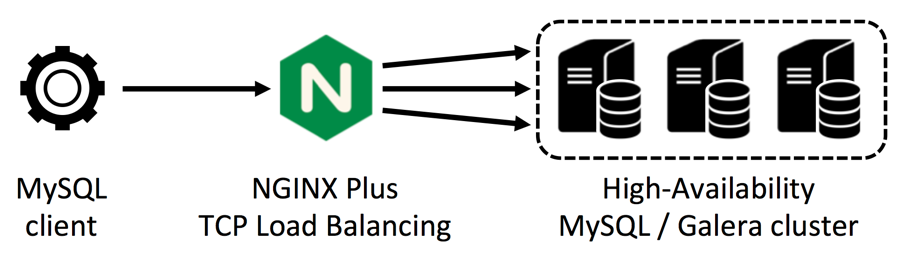
\includegraphics[width=\linewidth]{images/nginx-plus-load-balancing.png}
     \caption{Діаграма компонентів комунікації Nginx та Galera кластеру для MySql баз даних.}
     \label{fig:nginx_mysql}
\end{figure}

То ж, ми можем зробити висновок, що у цій архітектурі налаштування балансувальнику Nginx для комунікації с базами даних можлива. Подібні рішення будут працювати і з Mongo DB, Postgres, Percona та іншими. 

Теперь ми пропонуємо розібратись, чи підтримує Nginx динмічне балансування. 
Nginx PLUS реалізує динамічне балансування за допомогою груп серверів (upstream servers) таким чином: конфігурація серверів у групі може змінбватися динамічно за допомогою Nginx Plus REST API інтерфейсу. Адміністратор мережі може дивится сервери у групах або передивится конфігурацію конкретного серверу, змінювати параметри серверу, а також додавати або видаляти сервери за допомогою HTTP запитів на NGINX Plus REST API.
Остання опція - це і є той ключ, який задовільняю потреби алгоритму. 

Тобто, наразі NGINX Plus підходить за всіма параметрами, але якщо знадобиться поширювати функціонал реалізації нашого основного механізму, це неможливо буде зробити на стороні NGINX Plus, бо NGINX Plus - комерційне забезпечення, хоча і є продуктом NGINX reverse proxy - веб-серверу з можливостями статичного балансування з відкритим джерелом коду. Хоча є можливість реалізувати інший модифікований протокол балансування для узгодженості в NGINX proxy, але це потребує й реалізації алгоритму динамічного балансування, бо NGINX proxy підтримує тільки статичні алгоритми. Для цього приведемо порівняльну характеристику Nginx - Nginx Plus
(http://linuxbsdos.com/2015/09/25/nginx-plus-vs-open-source-nginx/ ) (див.\ref{fig:nginx_nginx_plus} )

\begin{figure}
\centering
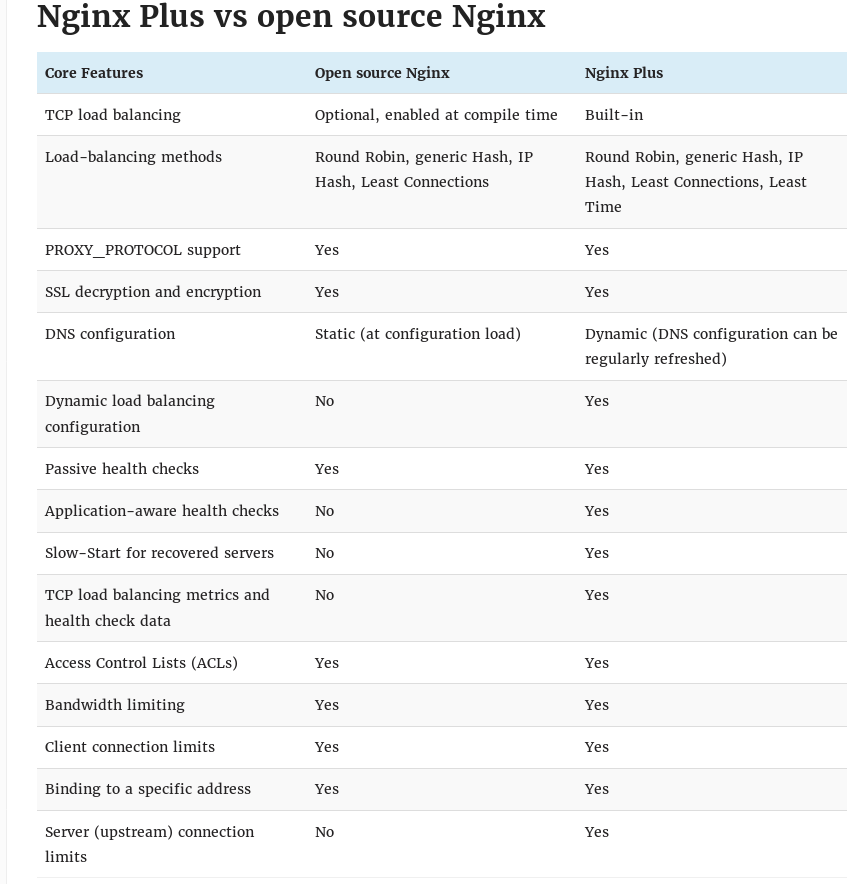
\includegraphics[width=\linewidth]{images/compare_nginx_nginx_plus.png}
     \caption{Порівняльна характеристика можливостей балансування навантаження у Nginx та NGINX Plus.}
     \label{fig:nginx_nginx_plus}
\end{figure}

\subsection{HAProxy}

HAProxy - програмне забезпечення з відкритим джерелом коду, проксі-сервер з високим рівнем доступності, який підтримує балансування в системі HTTP/TCP серверів, в тому числі і динамічне.
HAProxy забезпечує комунцікацію з базами даних за схожим принципом, що і NGINX Plus. Наступна діаграма компонентів описує один із прикладів архітектури, яку можуть побудувати адміністратори мережі розподіленої бази даних (див. Малюнок \ref{fig:haproxy_mysql}):

\begin{figure}
\centering
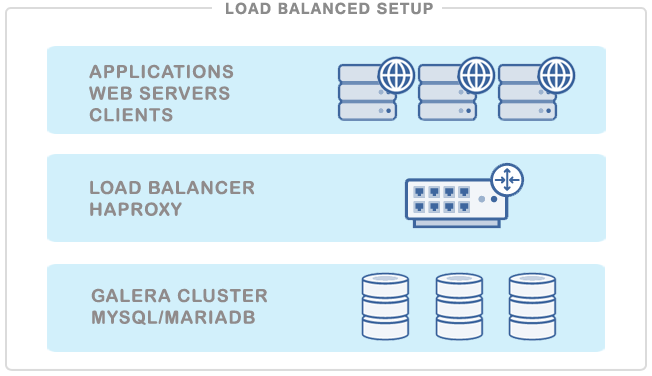
\includegraphics[width=\linewidth]{images/haproxy_database_balancing.png}
     \caption{Діаграма компонентів комунікації HAProxy з вузлами бази даних MySQL}
     \label{fig:haproxy_mysql}
\end{figure}


Оскільки HAProxy - найбільш потужна реалізація балансувальника навантаження, ми можем роздивитись діаграму компонентів більш детально для огляду можливостей, які можуть стати нам у нагоді.

Клієнтська програма, яка спирається на базу даних на "бекенді" (вузел, який відповідає за серверну частину виконання запиту), може легко переповнити базу даних багатьма запланованими паралельними з'єднаннями. HAProxy забезпечує чергу та регулявання підключень до одного або декількох серверів MySQL і запобігає перевантаженню одного сервера надто великою кількістю запитів. Всі клієнти підключаються до примірника HAProxy, а зворотний проксі-сервер (reverse proxy) пересилає з'єднання з одним з доступних серверів MySQL на основі алгоритму балансування завантаження.

За допомогою HAProxy в класі балансування навантаження ви матимете наступні переваги:

\begin{itemize}
\item Усі програми мають доступ до кластера за допомогою однієї IP-адреси або імені хосту. Топологія кластеру баз даних маскується за HAProxy.
\item З'єднання MySQL є збалансованими між завантаженими вузлами БД.
\item Можна додавати або видаляти вузли бази даних без будь-яких змін у програмах. 
\item Після досягнення максимальної кількості з'єднань в базах даних (в MySQL), HAProxy чергує додаткові нові підключення. Це добре зроблений спосіб регулювання запитів на з'єднання з базою даних і забезпечує захист від перевантажень.

\end{itemize}

ClusterControl підтримує розгортання HAProxy одразу з інтерфейсу користувача, і за замовчуванням він підтримує три алгоритми балансування навантаження - roundrobin, least connection або source. Користувачам рекомендується мати HAProxy між клієнтами та пулом серверів баз даних, особливо для кластерів Galera або MySQL Cluster, де запити на "бекенди" обробляються однаково.

Також можна налаштувати перевірку HAProxy, яка перевіряє, чи підключений сервер, просто підключившись до порту MySQL (як правило, 3306).

Найкращий спосіб перевірки здоров'я MySQL - це використання власного сценарію ("скрипт" у цьому випадку), який визначає наявність сервера MySQL, ретельно вивчаючи його внутрішній стан, який залежить від використовуваного рішення кластеризації. За замовчуванням ClusterControl надає власну версію сценарію перевірки здоров'я, яка називається mysqlchk, яка розташована на кожному сервері MySQL у наборі балансування навантаження, і має можливість повернути статус HTTP-відповіді та (або) стандартний вихід (stdout), який корисний для перевірки стану здоров'я на рівні TCP.

\textbf{ mysqlchk для Galera Cluster}. Якщо сервери сервера MySQL пройшли перевірку стану, то скрипт поверне простий HTTP 200 код статусу OK зі статусом виходу 0. А інакше скрипт поверне 503 Сервіс недоступний і статус завершення 1.
Використання $xinetd$ - це найпростіший спосіб отримати сценарій перевірки стану здоров'я, зробивши його демоном та прослуховуючи спеціальний порт (за замовчуванням - 9200). Після цього HAProxy підключиться до цього порту і запитає про вихід перевірки здоров'я. Якщо метод перевірки стану - httpchk, HAProxy буде шукати код відповіді HTTP, і якщо метод tcp-check, він буде шукати очікуваний рядок.

Наведена нижче блок-схема ілюструє процес звітування про стан здоров'я вузла Galera для встановлення декількох майстрів (див. \ref{fig:mysqlchk}).

\begin{figure}
\centering
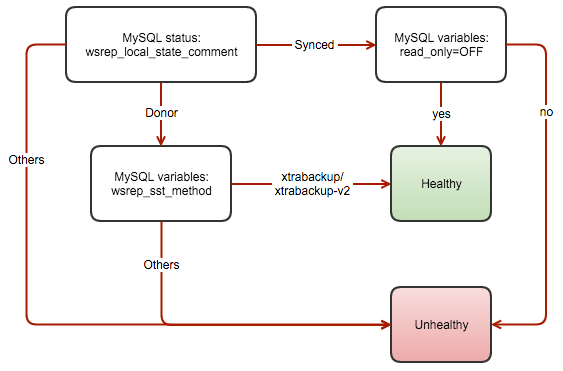
\includegraphics[width=\linewidth]{images/mysqlchk.png}
     \caption{Діаграма активності перевірки працездатності (healthcheck) вузлу бази даних з наявністю налаштованого HAProxy серверу}
     \label{fig:mysqlchk}
\end{figure}

https://severalnines.com/resources/tutorials/mysql-load-balancing-haproxy-tutorial

Відповідно до того, що сказано вище (стаття [18]) , є можливість для адміністратора мережі написати власну реалізацію перевірки працездатності для бази даних, тобто таблиця здорових (в нашому випадку, здорових і узгоджених) вузлів буде змінюватися за цим алгоритмом. 

Варто зауважити, що перевірка працездатності виконується HAProxy з конфігурованою періодичністю, 
тобто адміністратор розподіленої мережі бази даних також може цим керувати.


HAProxy, як і NGINX Plus , підтримує конфігурацію кластерів серверів, тобто відповідні одиниці даних сервери можуть бути об'єднані у кластери. 
Для цього потрібно сконфігурувати необхідну кількість бекендів, де кожний бекенд (backend) може відповідати за кластер. 

Також HAProxy реалізує механізм, відомий як комутація на основі контенту, який реалізується за 
допомогою контрольного списку доступу (ACL - Access Control List).
Спершу зробимо визначення ACL:

Більшість операцій у HAProxy можуть бути виконаними з певними умовами. Ці умови будуються через комбінації кількох контрольних списків доступу, використовуючи логічні оператори (AND, OR, NOT). Кожний такий список є серією тестів, які основані на таких елементах:

\begin{itemize}

\item спосіб вилучення методу для вилучення елемента для тестування; ;

\item необов'язкова серія перетворювачів для перетворення елемента ;

\item список відповідних шаблонів ;

\item відповідний метод, який вказує, як порівнювати шаблони із зразком

\end{itemize}

Тепер вертаєючись до механізму комутації контенту, можемо описати і його: принцип цього механізму полягає у наступному: 
коли відбувається з'єднання (connection) або запит (request) , запит або з'єднання містить в собі деяка інформацію, яка може впливати на те, який бекенд (група вузлів) буде вибраний для цього запиту. Це реалізується за допомогою умов на основі ACL. Тобто якщо інформація, яку містить запит чи з'єднання, відповідає умовам ACL, то може бути вибраний певний бекенд.


Отже, ми можемо побачити, що HAProxy має надзвичайно гнучку конфігурацію, що дозволяє нам сформувати відповідну модель роботи з балансуванням навантаження між узгодженими вузлами для певної одиниці даних.

\subsection{Інші балансувальники}

Ми роздивилися найбільш популярні, потужні, багатофункціональні балансувальники навантаження  з гнучкою конфігурацією. Але є інші балансувальники, які теж варті уваги. Ми оглянемо їх у цьому підрозділі і вирішимо, чи існує можливість використовувати їх для меїанізму балансування між узгодженими вузлами.
\begin{itemize}

\item Seesaw. Це балансувальник навантаження, розроблений компанією Google. Проблема полягає в тому, що цей балансувальник задовільняє лише потреби Google. Але так чи інакше він не має такого гнучкого функціоналу для того, щоб конфігурувати систему балансування за нашими вимогами. [30]
https://opensource.googleblog.com/2016/01/seesaw-scalable-and-robust-load.html

\item Traefik. Traefik - це сучасний HTTP зворотній проксі-сервер для мікросервісів. Traefik легко інтугрується з існуючим стеком компонентів інфраструктури в системі (Docker, Swarm mode, Kubernetes, Marathon, Consul, Etcd, Rancher, Amazon ECS, ...) і налаштовується автоматично і динамічно. Опція 
and configures itself automatically and dynamically. Pointing Traefik на компоненти оркестрації - це єдиний необхідний крок налаштування. Але Traefik не підтримує балансування для баз даних, та не може бути задіяний у використанні з іншими компонентами, які будуть служити посередниками між Traefik та вузлами бази даних.
https://docs.traefik.io/

\item Neutrino. Neutrino - розробка eBay PaaS команди. Neutrino повторює у багатьох елементів функціональності HAProxy, бо перед тим, як розробляти цей балансувальник команда eBay стояли перед вибором: віддати перевагу рішенню HAProxy чи розробити власний балансувальник.  [31]
https://www.ebayinc.com/stories/blogs/tech/announcing-neutrino-for-load-balancing-and-l7-switching/ . Рішення розробити Neutrino було вибрано за таких причин:
HAProxy не задовільнив вимогам для комутації між вузлами на рівні HTTP, базуючись на деяких специфічних правилах, 
відправки журналу повідомлень на кінцеві точки (endpoints) API (Application programming interface) , а також можливість додавання нових алгоритмів балансування.

Завдяки тому, що Neutrino, як і HAProxy, підтримує балансування і на рівні HTTP, і на рівні TCP, може бути використане рішення кластеру Galera, 
та приклад диаграми компонентів може мати такий самий вигляд, як і для HAProxy та NGINX Plus (див. Малюнки \ref{fig:haproxy_mysql} та \ref{fig:nginx_mysql}).
Окрім того, Neutrino - також рішення з відкритим джерелом коду, єдиний недолік - це те, що Neutrino підтримує менш функціоналу, ніж HAProxy та NGINX Plus, і механізм балансування між узгодженими вузлами, використаний разом з цим балансувальником, може мати більшу складність. 

\end{itemize}

Отже, з балансувальників, які ми роздивилися, ми можемо вибрати три, реалізувати математичні та імітаційні моделі, в яких одним з компонентом буде той чи інший балансувальник. 


Також у наступних розділах робиться оцінка кожної моделі. Також доведемо, що моделі, які містять тільки компоненти з програмного забезпечення балансувальників та повністю реалізують потрібний нам механізм, не існують.

Між тим ми розглянемо варіант моделі розподіленої бази даних, яка зовсім не має в якості компоненту жодного програмного забезпечення балансування навантаження, визначимо переваги та недоліки такої моделі і також зробимо її оцінку.

В кінці кінців це допоможе нам зробити оптимальне рішення та вибрати модель, яка найбільш відповідає нашим вимогам і має найменший показник складності алгоритму, який може бути реалізований за цією моделлю.

\section{Хеш-таблиці для зберігання узгоджених вузлів}

Перед тим, як приступити к моделюванню розподіленої баз даних з участю механізму балансування між ухгодженими вузлами, також необхідно зробити визначення рішення хеш-таблиць та роль яка відводиться їм у рішеннях з балансуванням. 

Отже, {\bfseries Хеш-таблиця } або {\bfseries хеш-відображення } - структура даних, що реалізує інтерфейс асоціативного масиву, а саме, вона дозволяє зберігати пари (ключ, значення) і здійснювати три операції: операцію додавання нової пари, операцію пошуку і операцію видалення за ключем. Існує два основних варіанта хеш-таблиць: з ланцюжками і з відкритою адресацією. Хеш-таблиця містить в собі деякий масив H, елементами якого є пари (хеш-таблиця з відкритою адресацією) або списки пар (хеш-таблиця з ланцюжками).

Виконання операцій в хеш-таблиці починається з обчислення хеш-функції від ключа. Отримане хеш-значення i = hash(key) відіграє роль індексу в масиві H. Після цього операція (додавання, видалення, пошук) перенаправляється об'єктові, який зберігається у відповідній комірці масиву H[i].

Ситуація, коли для різних ключів отримується одне й те саме хеш-значення, називається колізією. Такі події непоодинокі — наприклад, при додаванні в хеш-таблицю розміром 365 комірок усього лише 23-х елементів ймовірність колізії вже перевищує 50 відсотків (якщо кожний елемент може з однаковою ймовірністю потрапити в будь-яку комірку)  — див. парадокс днів народження. Через це механізм розв'язання колізій — важлива складова будь-якої хеш-таблиці.

В деяких особливих випадках вдається взагалі уникнути колізій. Наприклад, якщо всі ключі елементів відомі заздалегідь (або дуже рідко змінюються), тоді для них можна знайти деяку досконалу хеш-функцію, яка розподілить їх за комірками хеш-таблиці без колізій. Хеш-таблиці, які використовують подібні хеш-функції, не потребують механізму розв'язання колізій, і називаються хеш-таблицями з прямою адресацією. 

Роздивимося хеш-таблицю більш детально: 

\paragraph{\textbf{Постановка задачі}}
[36] 
%http://elcat.pnpu.edu.ua/docs/%D0%90%D0%BB%D0%B3%D0%BE%D1%80%D0%B8%D1%82%D0%BC%D0%B8%20%D1%96%20%D1%81%D1%82%D1%80%D1%83%D0%BA%D1%82%D1%83%D1%80%D0%B8%20%D0%B4%D0%B0%D0%BD%D0%B8%D1%85/lab12-13_table.html
У хеш-таблиці замість безпосереднього використання ключа як індексу масиву, індекс обчислюється за значенням ключа. 
Функція, що відображає елемент множини ключів ${0, 1, ..., n-1}$ на множину індексів ${0, 1, ..., m-1}$, $(m <n)$, 
називається хеш-функцією. 
Якщо два ключі хешуються в одну й ту саму комірку, то говорять про виникнення колізії. За способом вирішення колізій розрізняють:
\begin{itemize}
\item відкрите хешування — усі елементи, що хешуються в одну комірку, об’єднуються у зв’язний список. При відкритому хешуванні хеш-таблиця є масивом, кожна комірка якого містить покажчики на заголовок списку всіх елементів, хеш-значення ключа яких дорівнює індексу комірки. 
\item закрите хешування — усі елементи зберігаються безпосередньо у хеш-таблиці, при потраплянні у зайняту комірку обирається послідовність інших хеш-значень. 
При закритому хешуванні хеш-таблиця є масивом, елементи якого занумеровані від 0 до m-1.
\end{itemize}


Необхідно забезпечити для хеш-таблиці реалізацію основних операторів:
\begin{itemize}
\item пошук елемента;
\item запис елемента;
\item читання елемента. 
\end{itemize}

\paragraph{Існуючі рішення для хеш-таблиць}

\section{Моделі власного механізму та його оцінка}
В цьому розділі ми зробимо концептуальні моделі та моделі компонентів для рішення маршрутизації між узгодженими нодами без задіяння відомого програмного забезпечення балансувальників навантаження, щоб мати повну картину для оцінювання у подальших розділах.

Зараз ми представляємо математичну модель для розподіленої бази даних.
Ми визначаємо її як кортеж компонентів $(N, L, \partial,D, r)$, де \\

\begin{tabular*}{\textwidth}{cp{0.5cm}p{0.8\textwidth}}\label{tb:mm_first}
$N$&& - кінцева множина вузлів розподіленій бази даних; \\
$L$&& - кінцева множина посилань (зв'язків) між вузлами у розподіленiй базі даних; \\
$\partial:L\rightarrow 2^N$&& - відображення, яке  сполучає кожне посилання з двома вузлами у мережі розподіленої бази даних;\\
$D$&& - кінцева множина зберігаємих нероздільних одиниць даних залежачи від побудованої схеми розподіленої бази даних та принципу розподілення у тий чи іншій конфігурації;\\
$r:D\rightarrow 2^N$&& - відображення, яке ассоціює кожну одиницю даних $d$ з підмножиною вузлів, які зберігають репліку такої одиниці даних; \\

$R(d)$&& - кінцева множина реплік (версій) $r$ даної одиниці даних $d$;\\
$N(d)$&& - кінцева множина вузлів, які зберігають репліку даної одиниці даних $d$; \\
$l(N(d))$&& - кількість вузлів у розподіленій базі даних, які зберігають репліку даної одиниці даних $d$; \\
$n_c$&& - кількість вузлів підмножини $N_d$, де всі вузли зберігають одну і ту ж версію одиниці даних.

$D:$
\end{tabular*}

У цьому розділі ми розширимо існуючу модель визначенням:

\begin{definition}
$N(c, d)$ - кінцева множина вузлів підмножини $N(d)$, де всі вузли зберігають одну і ту ж версію одиниці даних, тобто одну і ту ж репліку. Це визначає множину вузлів, які узгоджені між собою відповідно до одиниці даних $d$.


\end{definition}

Цю модель найбільш точно відображує наступна діаграма компонентів (див. Малюнок \ref{fig:d_components_without_lb}).


\begin{figure}
\centering

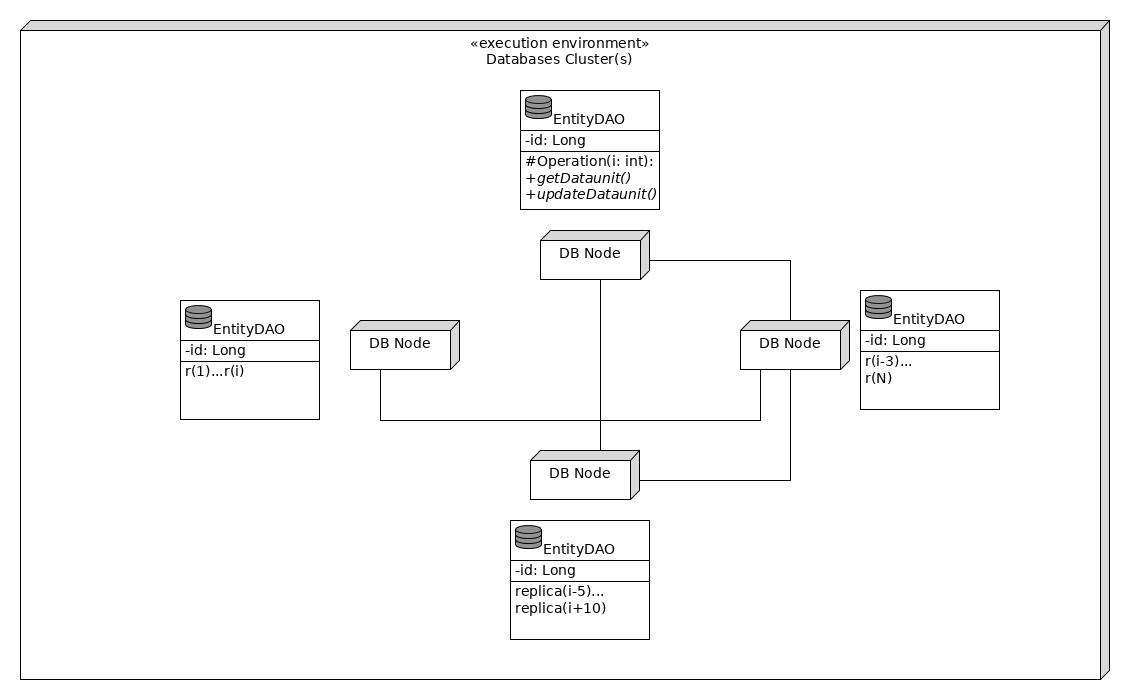
\includegraphics[width=\linewidth]{images/d_component_without_lb.jpg}
     \caption{Діаграма компонентів розподіленого сховища без балансувальника навантаження.}
     \label{fig:d_components_without_lb}
\end{figure}

Також ми представляємо концептуальну модель і діаграму послідовності, за допомогою яких буде будуватися імітаційна модель для цього зразку математичної моделі (див. Малюнок \ref{fig:d_concepts_without_lb} і Малюнок \ref{fig:d_sequence_without_lb})
\begin{figure}
\centering

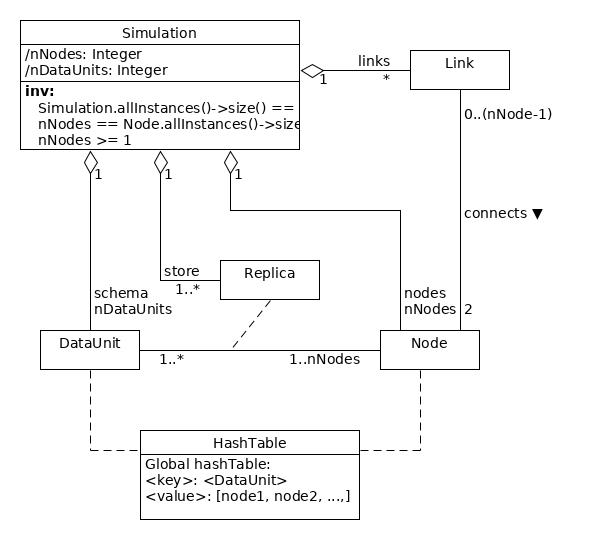
\includegraphics[width=\linewidth]{images/d_concept_without_lb.jpg}
     \caption{Діаграма концептів розподіленого сховища без балансувальника навантаження.}
     \label{fig:d_concepts_without_lb}
\end{figure}


\begin{figure}
\centering

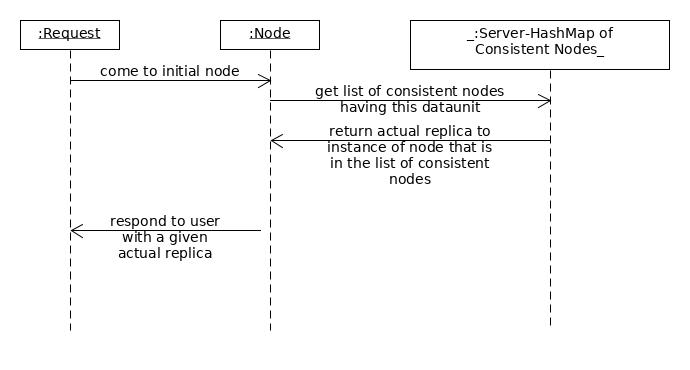
\includegraphics[width=\linewidth]{images/d_sequence_without_lb.jpg}
     \caption{Діаграма послідовності розподіленого сховища без балансувальника навантаження.}
     \label{fig:d_sequence_without_lb}
\end{figure}

Після побудування моделей, крім імітаційної, ми можемо зробити висновки про переваги та недоліки такого алгоритму:

\begin{itemize}
\item Переваги
\begin{itemize}
\item Незалежність від іншого програмного забезпечення, оскільки це рішення не використовує жодних сторонніх  глобальних рішень
\item Простота реалізації. Таке рішення не є ресурсо-витратним, щоб реалізувати такий алгоритм, потрібен сервер (кластер) с хеш-таблицею, яка буде містити список вузлів за конкретною одиницею даних (побудова такої таблиці може залежити від того, як одиниці даних розподілені між вузлами мережі розподіленого сховища)

\end{itemize}
\begin{itemize}
\item Ненадійність. Такий механізм не є надійним, бо неможливо гарантувати працездатність всіх узгоджених вузлів у хеш-таблиці, і так чи інакше цей алгоритм потребує періодичну перевірку стану вузлів, тому що з того часу, як вузел став узгодженим, він міг вийти із зони доступності. Зону доступності (availability) може гарантувати періодична перевірка стану вузлів. Однак такий механізм може використовуватися, якщо адміністратор мережі і бізнес-аналітики проекту, компонентом якого  розподілена база за цією моделлю, можуть гарантувати таку доступність вузлів та зв'язків між ними (або знайти рішення, яке буде це гарантувати), що після запиту на запис вузел не вийде з зони доступності, або запити на запис відбуваються з таким коротким інтервалом, що це до дозволить в цей же час перевіряти і стан вузлів одночасно с оновленням хеш-таблиці.
\item Залежність кожного вузла один від одного. Вузли повинні спілкуватися між собою за епідеміологічними алгоритмами
\end{itemize}
\end{itemize}

Щоб довести це, ми побудували імітаційну модель (див. Додатки) за побудованими раніше концептуальной діаграмою та діаграмою послідовності.

У якості глобальної Хеш-таблиці ми вибрали Redis (порівняльна характеристика різних рішень хеш-таблиць представлена у другому розділі поточної глави).

\section{Моделі гібрідного механізму з використанням балансувальника}
Побудувавши математичну, концептуальну та імітаційну модель у минулому розділі, ми будемо дотримуватися такої самої стратегії для гібрідного рішення.
Оскільки кожний балансувальник різний, що ми вже показали у першому розділі цієї глави, ми повинні врахувати цей факт при побудуванні моделей для цього рішення та, можливо, зробити кілька варіантів моделей для кожного з вибраних балансувальників. 

Першою моделлю, яку ми опишемо, стане модель для балансування між узгодженими вузлами, базуючись на програмному рішенні HAProxy.

Отже, модель розподіленої системи даних у цьому рішенні поширюється іншими компонентами, які необхідні для перевірки стану вузлів та балансування між ними.
Посилаючись на вже розроблену модель для розподіленої бази даних (див. Модель у минулому розділі \ref{tb:mm_first}), ми додаємо такі елементи:

\begin{tabular*}{\textwidth}{cp{0.5cm}p{0.8\textwidth}}\label{tb:mm_second}
$SLB frontend$&& - потужний сервер або група потужних серверів, які відповідають за балансування и мають встановлений сервер балансувальника HAProxy, відповідаючи за обробку запитів. Запит на запис повинен виконуватися таким самим чином, як би він виконувався у будь-якій розподіленій системі бази даних. У випадку запита на читання, балансувальник повинен опрацювати запит налаштованих умов контрольного списку доступу та направити запит на відповідний $SLB backend$;\\
$SLB backend$&& - кінцева множина кластерів для розподіленої бази даних, які повинні опрацювати запит.

\end{tabular*}

Тепер роздивимося спрощений варіант діаграми компонентів для цієї моделі (див. Малюнок \ref{fig:d_components_lb}). Варто зауважити, що для чистоти зображення на цій діаграмі не вказані зв'язки між вузлами, бо це відноситься до того принципу, як розповсюджуються репліки між вузлами мережі розподіленої бази даних, а не до механізму роботи кластера балансувальника та кластерів вузлів РБД. Однак цей факт буде відображений у наступній діаграмі. (див Малюнок \ref{fig:d_concept_lb}). 

\begin{figure}
\centering

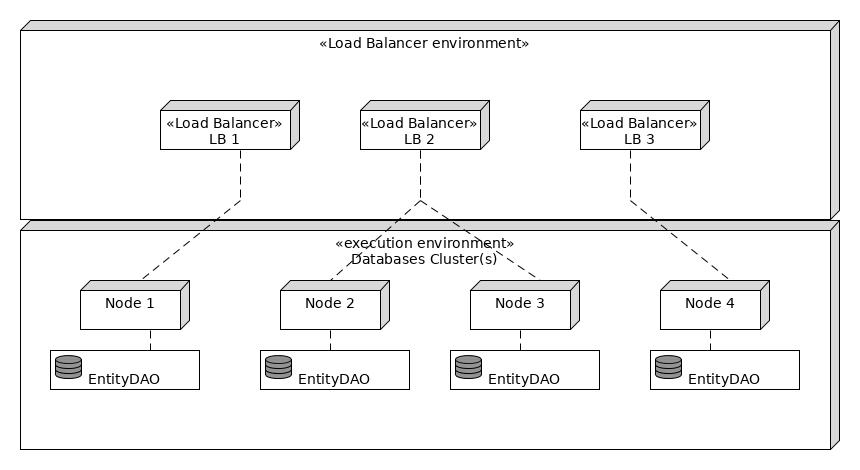
\includegraphics[width=\linewidth]{images/d_components_lb.jpg}
     \caption{Діаграма 	компонентів розподіленого сховища за участі балансувальника навантаження.}
     \label{fig:d_components_lb}
\end{figure}

\begin{figure}
\centering

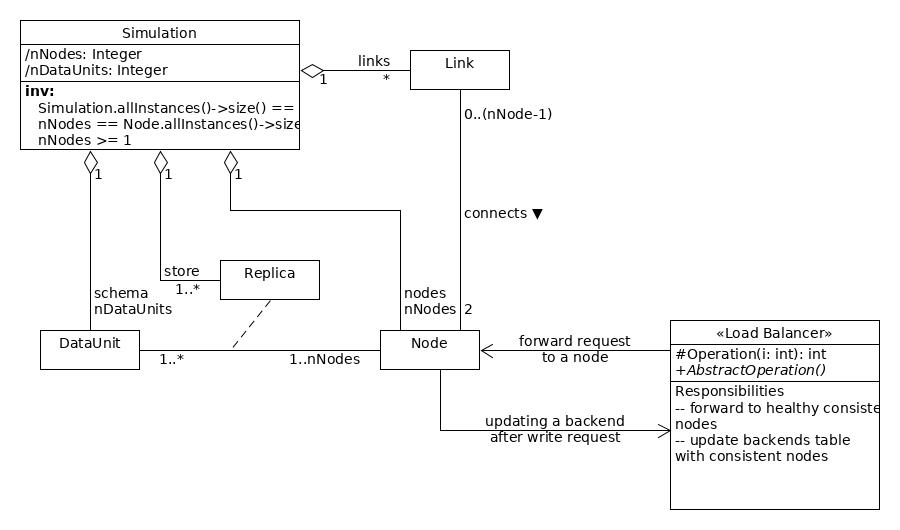
\includegraphics[width=\linewidth]{images/d_concept_lb.jpg}
     \caption{Діаграма 	концептів розподіленого сховища за участі балансувальника навантаження.}
     \label{fig:d_concept_lb}
\end{figure}


Наступні діаграми, яку хотілося б презентувати, є діаграми послідовності для розподіленого сховища даних за участі рішення балансувальника.
Ці діаграми розділені на кілька частин, де перша діаграма презентує програмне рішення для розподіленого сховища (див. Малюнок \ref{fig:d_sequence_lb}), а друга - інфраструктурне рішення, яке показує більш детально рекомендації для налаштування балансувальника навантаження

\begin{figure}
\centering

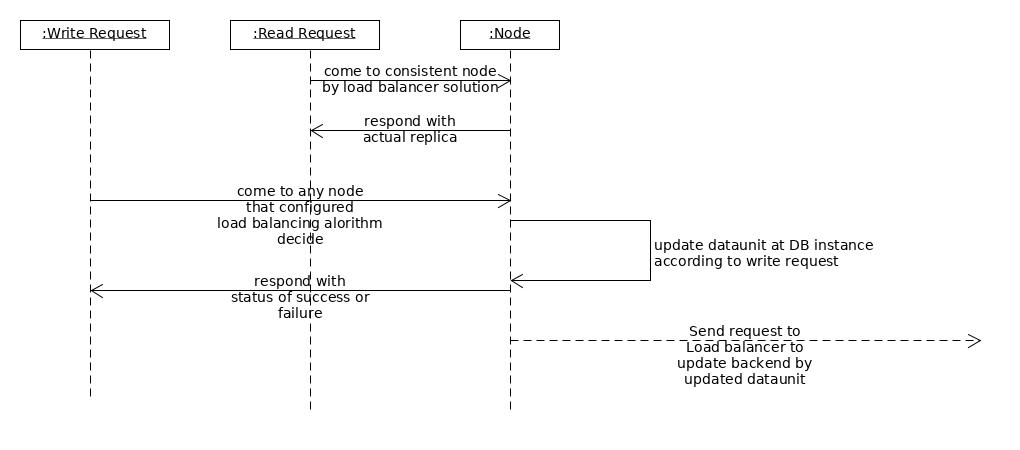
\includegraphics[width=\linewidth]{images/d_sequence_lb.jpg}
     \caption{Діаграма 	послідовності розподіленого сховища за участі балансувальника навантаження. Програмне рішення}
     \label{fig:d_sequence_lb}
\end{figure}

Наступні діаграми можуть мати декілька варіантів реалізації, оскільки ми описуємо можливості використання декількох реалізацій балансувальника навантаження,
і кожне з них може бути налаштовано зовсім різними методами, існуючими у той чи іншій реалізації. 


\section{Оцінка несуперечливості та доступності за застосованими моделями}


\chapter{Дослідження часу збіжності несуперечливості у ідеальному сховищі}

\chapter{Висновки}
\section{Потенціал використання моделей балансування узгодженості в розподілених сховищах даних}

\begin{thebibliography}{99}
% ---A---
\bibitem{bib:database_principles}
 — 
C.J. Date: 
An Introduction to Database Systems. 8th edition.
%
\bibitem{bib:database_integrity}
Г.Ладиженський:
Распределенные информационные системы и базы данных.
Конференция
http://citforum.ru/database/kbd96/45.shtml

\bibitem{bib:tanenbaum_distributed}
Aho, A. V., Sethi, R., Ullman, J. D.: 
Compilers: Principles, Techniques, and Tools (1st ed.). 
Addison-Wesley. ISBN 9780201100884 
(1986).
%
\bibitem{bib:algorithms_epidemic}
\bibitem{bib:algorithms_epidemic}


\end{thebibliography}
\end{document}
